% THIS IS SIGPROC-SP.TEX - VERSION 3.1
% WORKS WITH V3.2SP OF ACM_PROC_ARTICLE-SP.CLS
% APRIL 2009
%
% It is an example file showing how to use the 'acm_proc_article-sp.cls' V3.2SP
% LaTeX2e document class file for Conference Proceedings submissions.
% ----------------------------------------------------------------------------------------------------------------
% This .tex file (and associated .cls V3.2SP) *DOES NOT* produce:
%       1) The Permission Statement
%       2) The Conference (location) Info information
%       3) The Copyright Line with ACM data
%       4) Page numbering
% ---------------------------------------------------------------------------------------------------------------
% It is an example which *does* use the .bib file (from which the .bbl file
% is produced).
% REMEMBER HOWEVER: After having produced the .bbl file,
% and prior to final submission,
% you need to 'insert'  your .bbl file into your source .tex file so as to provide
% ONE 'self-contained' source file.
%
% Questions regarding SIGS should be sent to
% Adrienne Griscti ---> griscti@acm.org
%
% Questions/suggestions regarding the guidelines, .tex and .cls files, etc. to
% Gerald Murray ---> murray@hq.acm.org
%
% For tracking purposes - this is V3.1SP - APRIL 2009

\documentclass{acm_proc_article-sp}
\usepackage{url}

%
\def\sharedaffiliation{%
\end{tabular}
\begin{tabular}{c}}
%

\begin{document}


\title{UMD Event Finder, A Context-Aware Event Finder Application on Mobile Platform\titlenote{This effort is part of the CMSC818G, Information-Centric Design of Context-Aware Systems, class project.}}
%
% You need the command \numberofauthors to handle the 'placement
% and alignment' of the authors beneath the title.
%
% For aesthetic reasons, we recommend 'three authors at a time'
% i.e. three 'name/affiliation blocks' be placed beneath the title.
%
% NOTE: You are NOT restricted in how many 'rows' of
% "name/affiliations" may appear. We just ask that you restrict
% the number of 'columns' to three.
%
% Because of the available 'opening page real-estate'
% we ask you to refrain from putting more than six authors
% (two rows with three columns) beneath the article title.
% More than six makes the first-page appear very cluttered indeed.
%
% Use the \alignauthor commands to handle the names
% and affiliations for an 'aesthetic maximum' of six authors.
% Add names, affiliations, addresses for
% the seventh etc. author(s) as the argument for the
% \additionalauthors command.
% These 'additional authors' will be output/set for you
% without further effort on your part as the last section in
% the body of your article BEFORE References or any Appendices.

\numberofauthors{3} %  in this sample file, there are a *total*
% of EIGHT authors. SIX appear on the 'first-page' (for formatting
% reasons) and the remaining two appear in the \additionalauthors section.
%
\author{
% You can go ahead and credit any number of authors here,
% e.g. one 'row of three' or two rows (consisting of one row of three
% and a second row of one, two or three).
%
% The command \alignauthor (no curly braces needed) should
% precede each author name, affiliation/snail-mail address and
% e-mail address. Additionally, tag each line of
% affiliation/address with \affaddr, and tag the
% e-mail address with \email.
%
% 1st. author
\alignauthor Samet Ayhan\\
       \affaddr{University of Maryland, Department of Computer Science}\\
       \affaddr{College Park, Maryland 20740}\\
       \email{sayhan@cs.umd.edu}
% 2nd. author
\alignauthor Snigdha Chaturvedi\\
       \affaddr{University of Maryland, Department of Computer Science}\\
       \affaddr{College Park, Maryland 20740}\\
       \email{snigdhac@cs.umd.edu}
% 3rd. author
\alignauthor Adil Yalcin\\
       \affaddr{University of Maryland, Department of Computer Science}\\
       \affaddr{College Park, Maryland 20740}\\
       \email{adil.yalcin@gmail.com}
}
% There's nothing stopping you putting the seventh, eighth, etc.
% author on the opening page (as the 'third row') but we ask,
% for aesthetic reasons that you place these 'additional authors'
% in the \additional authors block, viz.

\date{9 May 2013}
% Just remember to make sure that the TOTAL number of authors
% is the number that will appear on the first page PLUS the
% number that will appear in the \additionalauthors section.


\maketitle
\begin{abstract}
Context-aware event finding system is expected to make use of not only user preferences but also information surrounding the specific contextual situation that is relevant. For instance, a user in search of an event within a certain distance should be presented with a set by taking her current location into account. In fact, not only her current location, but also the distance specified, her preferences, and any other factors that help define the relevant context. This contextual information gathering ought to occur pervasively in an ever changing environment where the process is encapsulated from the user.

In this paper, we describe a novel mobile application that presents events on University of Maryland (UMD) College Park Campus to the user based on contextual information in addition to choices the user made in the past. The obvious challenge with this approach is determining and making use of the relevant contextual information per use-case. Experimental results appear to support that our application is able to efficiently and effectively present relevant events to the user on agnostic mobile platforms.
\end{abstract}

% A category with the (minimum) three required fields
\category{H.m}{Information Systems}[Miscellaneous], {H.3.4}{Information Storage and Retrieval}[Systems and Software—Distributed systems], {H.3.5}{Information Storage and Retrieval}[Online Information Services—Web-based services]

\terms{Design, Human Factors}

\section{Introduction}
According to the International Telecommunication Union (ITU), the number of cell phone subscribers has reached six billion in 2011, and mobile broadband subscriptions have exceeded one billion globally \cite{itu:cellphone}. Recent mobile phones provide users with a number of features such as Wi-Fi connectivity, bluetooth and GPS localization, camera and video capture devices and, additionally, the capacity for users to program the mobile devices with more applications. Among the most popular applications there are location-based services (LBSs), in which knowledge of the end user’s location is used to deliver relevant, timely, and engaging content and information \cite{rao:lbs}. As it is clear that location is not the only information defining the context. Time and any other information pertaining to the situation is considered part of contextual information. 

Most web applications today expose themselves with static interfaces in a segregated manner, where search options are presented to the user requiring her to make selections over and over again per session, without taking advantage of surrounding contextual information. Whereas ubiquitous and pervasive computing teaches better integration, systems to make use of contextual information. This way, users are presented with more accurate and timely information without requiring them to provide information that sensors already provide.

With these facts in mind, we have built a system that utilizes contextual information to serve for the purposes of event finding application on agnostic mobile platforms. Some of the key features are:
\begin{itemize}
\item Provided with Wi-Fi connectivity, any mobile device with a browser to invoke our service.
\item No matter what type of mobile device is used, all capabilities offered by the service as well as the look and feel to be identical. 
\item In addition to regular event search options, distance proximity and temporal queries are supported. 
\item Queries in previous sessions, presumably reflecting user's profile are stored for smarter recommendations. 
\end{itemize}

Furthermore, our application implements Model View Controller (MVC) architecture pattern, where the representation of information is segregated from the user's interaction with it. With this architecture approach, the model that consists of event data and the controlling business logic and the graphical user interface are all separated from each other so that loose coupling, better reusability and more scalable solution is attained.

Among other tools and technologies, our implementation made use of HTML5, JQuery, Python, MySQL, and Apache HTTP Server.

The rest of this paper is organized as follows: In Section 2, we present related work, in Section 3, we explain the architecture in addition to design and implementation of three main components, front-end, back-end, and the controlling business logic. In Section 4, we discuss some major use-cases, limitations and optimizations. The final section contains concluding remarks and future work.

\section{Related Work}
Plenty of research has been done in the area of context-aware computing in the past. Among these efforts, context-awareness has been mainly studied in the fields of ubiquitous, pervasive or mobile computing. Furthermore, a significant number of applications have been
successfully developed and deployed. 

Peddemors et al. introduce the PLIM framework which provides an infrastructure for the distribution and retrieval of location information of mobile devices using a publish/subscribe mechanism \cite{peddemors:lbs}.

Harter et al. describe a system that builds a dynamic model of the environment where location information for the objects are updated based on data received from sensors. Also, an event-based monitoring system is provided allowing applications to detect location changes \cite{harter:anatomy}. 

Indulska et al. present a context model for pervasive systems based on the CC/PP standard and points out some limitations of this standard  \cite{indulska:ccpp}.

In the Web service area, a number of work dealing with context has been done. The CB-SeC framework is an agent-based architecture that provides service selection based on a rating for Web services. The ratings are calculated using context of interest functions \cite{maamar:contextualisation}. 

Aura is an architectural framework that models user tasks as coalitions of abstract services. Aura migrates such tasks from one environment to another one when the user changes location. Also, tasks can be adjusted when the environment changes \cite{sousa:mobility}

In the information systems area, preferences are attracting noticeable attention due to fact that they are a means to support personalization within Web services, particularly within information services that often use DBMS as back-end. Preferences, also called soft constraints, are considered as wishes: The result of a query should be a perfect match, but a best possible match is also acceptable \cite{kießling:optimizing,agrawal:preferences,chomicki:intrinsic}.

Among the very first ones, with "The Insider" web application, students were able to keep up with happenings at the Arizona State University campus. Similar to our system, yet missing very key features, this system brought Mesa's Williams Campus together on PC as well as mobile devices \cite{valenzuela:insider,gellersen:multisensor}.

In the area of mobile computing, a number of papers discuss the effect of context on mobile usability, propose an expanded model of mobile application context, and conduct an empirical study to test a number of hypotheses concerning the use of software implementation technology and location context in mobile applications \cite{ryan:mobile}.

In their work, Alberto et al. analyse the prerequisites and enablers for context-aware mobile services. According to them,  the user perspective, the business perspective, as well as the required technological enablers need to be understood in order to make context-aware services a reality \cite{alberto:usercentric}.

With their research, Raptis et al. review mobile applications used in museum environments, focusing on the notion of context and its constituent dimensions \cite{raptis:museum}.

\section{Architecture}
In this section, we introduce the system architecture in detail. Although subsequent sections provide more detail regarding each component, here we will provide 10000 feet view.

Illustrated in Figure 1, UMD Event Finder Service utilizes a persistent storage, where events and other relevant information are stored. The data is periodically pulled from disparate data sources in various formats by invoking live feed consumption modules. The service is composed of a number of query modules such as geo-location, temporal, etc. The service makes use of these additional information by contacting corresponding sensors pervasively and incorporating the returned results in its query process. This process is completely encapsulated from the user. Upon search invocation from the end user, the service pulls all necessary pieces together and presents the results back to the user in an efficient and effective manner. The returned results can be viewed on any mobile platform or PC environment with the same look and feel.

\begin{figure*}
\centering
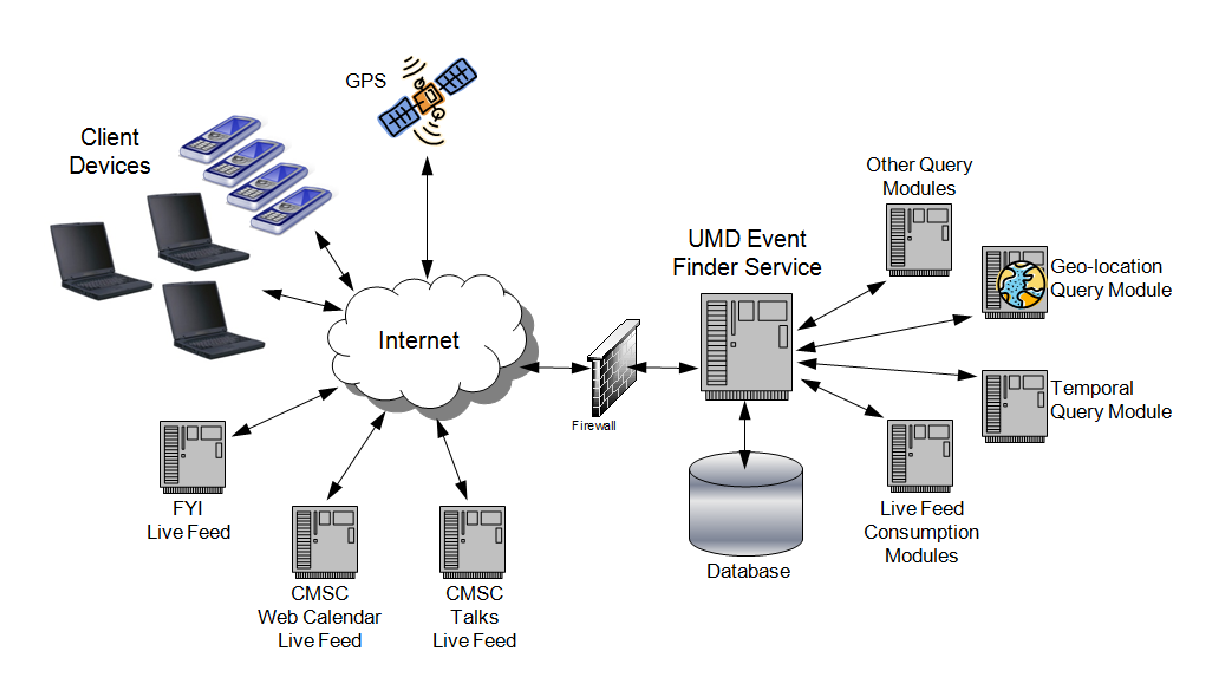
\epsfig{file=figure1.eps,height=3.7in,width=6.6in}
\caption{UMD Event Finder - Physical Architecture.}
\end{figure*}

\subsection{Front-end}	 
We explain front-end here...

\subsubsection{Back-end}
We explain back-end here...

\subsubsection{Business Logic}
We explain business logic here...

\section{Use-Cases and Discussion}
Use-cases and discussion go here...

\section{Conclusion and Future Work}
This paper introduced a novel system that presents UMD events on agnostic mobile platforms based on contextual information in addition to user preferences. Taking major contextual information into account such as location and time in an ever changing environments, our system retrieves relevant events and presents to the user in an efficient and effective way.

This very first version of our system delivers context-based services by contacting sensors pervasively and making use of every bit of relevant information for the events being sought. However, there is still room for improvement. Among others, authentication, persistent user profiles, integration with social media, and automated notifications using pub-sub pattern are all critical capabilities that may be developed.  

\section{Acknowledgments}
We would like to thank Brooke Supple for allowing us to connect with IT resources. We would also like to thank Skip Warnick and Brian Swartzfage​r for their help in providing us with access to the UMD FYI Events live feed. We thank all of the anonymous contributors. We would especially like to thank Dr. Agrawala for his advice and directions.

%
% The following two commands are all you need in the
% initial runs of your .tex file to
% produce the bibliography for the citations in your paper.
\bibliographystyle{abbrv}
\bibliography{sigproc}  % sigproc.bib is the name of the Bibliography in this case
% You must have a proper ".bib" file
%  and remember to run:
% latex bibtex latex latex
% to resolve all references
%
% ACM needs 'a single self-contained file'!
%
%APPENDICES are optional
%\balancecolumns
\balancecolumns
% That's all folks!
\end{document}
